\documentclass[../main.tex]{subfiles}
\begin{document}

A multilayer perceptron was implemented by modifying the appended Tensorflow code for a XOR gate. The authors wanted to use as few neurons possible, so the Tensorflow Playground \cite{tfpg} was applied. An outline of the neural net implemented is shown in \autoref{fig:mlp}. The authors were able to achieve decent results with only one hidden layer! A learning rate chosen was 
\begin{equation}
    \alpha = \vari{lr}
\end{equation}
The resulting cross-entropy error for training and testing is shown in \autoref{fig:cee}. 

\begin{figure}
    \centering
    \begin{subfigure}[b]{0.48\textwidth}
    	\centering
	    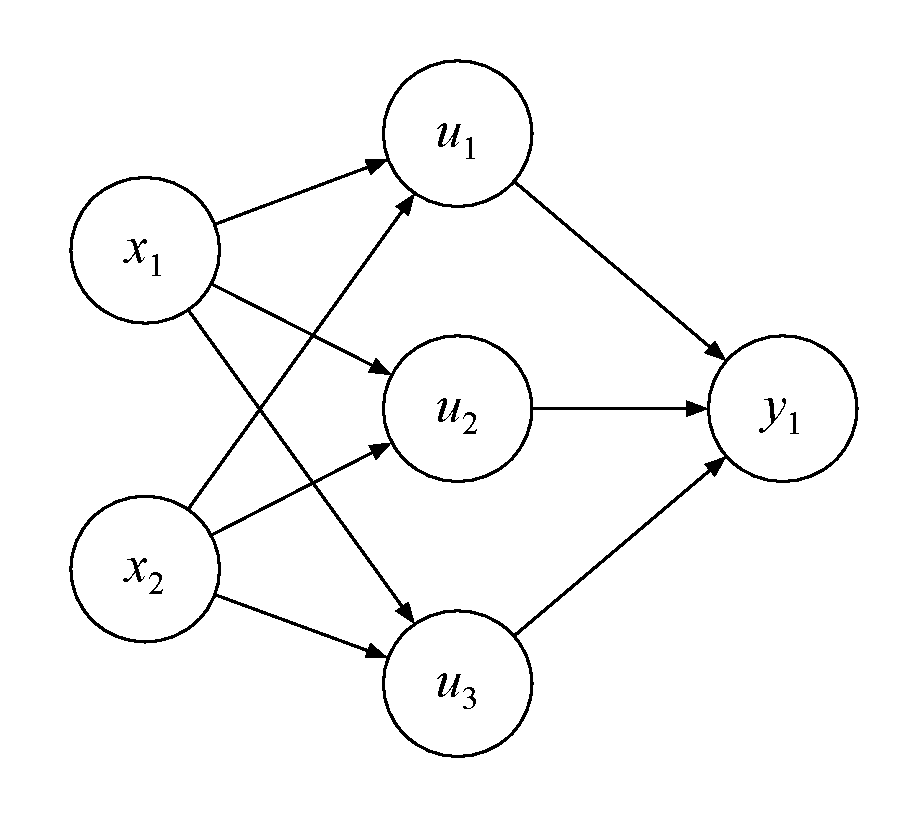
\includegraphics[width=\textwidth]{figures/mlp/mlp}
	    \caption{Neural network used for Multilayer Perceptron}
	    \label{fig:mlp}
    \end{subfigure}
    ~
    \begin{subfigure}[b]{0.48\textwidth}
    	\centering
        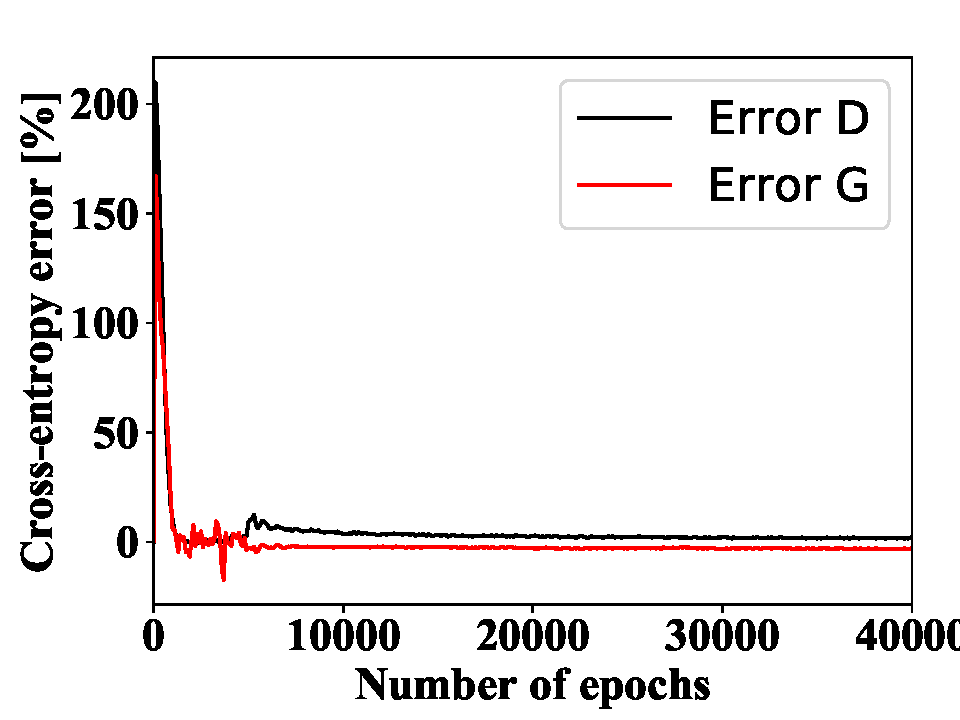
\includegraphics[width=\textwidth]{figures/mlp/cross_entropy_error}
        \caption{Cross entropy error of training and test data}
        \label{fig:cee}
    \end{subfigure}
    \caption{Neural network graph and cross entropy error for a Multilayer Perceptron.}
\end{figure}

\end{document}